% this is a comment in latex
% substitute this documentclass definition for uncommented one
% to switch between single and double column mode
\documentclass[11pt,twocolumn]{article}
%\documentclass[11pt]{article}

\usepackage{fullpage}
\usepackage{subfigure,indentfirst}
% for url
\usepackage{hyperref}
% for underlined text
\usepackage[normalem]{ulem}
% for including pdf figures
\usepackage{graphicx}

% my own versions: my_enumerate and my_itemize
\newenvironment{my_enumerate}{
  \begin{enumerate}
    \setlength{\itemsep}{1pt}
      \setlength{\parskip}{0pt}
\setlength{\parsep}{0pt}}{\end{enumerate}
}

\newenvironment{my_itemize}{
  \begin{itemize}
    \setlength{\itemsep}{1pt}
      \setlength{\parskip}{0pt}
\setlength{\parsep}{0pt}}{\end{itemize}
}

% this starts the document
\begin{document}

\title{CS87 Project Report: 
Integrating CUDA and MPI for Discrete Event Simulation}

\author{Hoang "Tommy" Vu, Dzineon Gyaltsen, Henry Lei, Sean Cheng \\
Computer Science Department, Swarthmore College, Swarthmore, PA  19081}

\maketitle

\begin{abstract}

In the evolving landscape of parallel programming, optimizing resource usage and 
leveraging system architectures remain two critical priorities. In this paper, we present the results of our investigation into an integration of the Open Message Passing Interface (OpenMPI) and Compute Unified Device Architecture (CUDA) platforms. Traditionally, CUDA and OpenMPI have been employed separately with CUDA excelling in GPU-based parallel execution but limited by GPU resources and OpenMPI facilitating inter-node communication without direct GPU utilization. These two platforms individually have shown improvements in high-performance simulation applications, yet little research has been done on the performance analysis of a CUDA-integrated OpenMPI hybrid model. Our study bridges this gap by implementing a parallel discrete event simulation task via Conway's Game of Life (GOL) across three parallel programming models: standalone CUDA, standalone OpenMPI, and the novel CUDA-OpenMPI hybrid.

The core of our research lies in the comparative analysis of runtime performance across these models, particularly under varying board sizes in GOL. Our findings reveal a nuanced performance landscape: while CUDA outperforms OpenMPI on smaller boards due to its efficient parallel processing, OpenMPI gains the upper hand on larger boards where CUDA's resource limitations become apparent. Significantly, the hybrid MPI-CUDA model demonstrates superior scalability, maintaining efficiency on larger boards where standalone CUDA is constrained by memory and data transfer overheads. The research conclusively demonstrates that although MPI-CUDA may not always surpass standalone CUDA in smaller contexts, it consistently outperforms standalone MPI and is essential for optimal performance on larger scales. This investigation not only underscores the strengths and limitations of CUDA and OpenMPI but also highlights the promising avenue of their combined usage in high-performance computing.

\end{abstract}


\section{Introduction}

Parallel programming has become a cornerstone in high-performance computing, addressing the ever-growing demand for computational efficiency and scalability. Among the prominent frameworks in this domain, Open Message Passing Interface (OpenMPI) and Compute Unified Device Architecture (CUDA) stand out. OpenMPI excels in facilitating communication between computing nodes for parallel processing, yet it does not inherently tap into the computational prowess of Graphics Processing Units (GPUs). On the other hand, CUDA leverages the vast parallelism capabilities of GPUs but is constrained by the finite resources of individual GPUs and nodes. This dichotomy presents a unique opportunity: the integration of CUDA and OpenMPI, potentially harnessing the strengths of both to elevate performance in parallel computing tasks.

This research aims to explore and quantify the performance of a hybrid CUDA-OpenMPI interface, particularly in the context of discrete-event simulation. Conway's Game of Life (GOL), chosen for its suitability for parallel execution, serves as the testbed for our experiments. We implemented GOL using three distinct parallel programming models: CUDA, OpenMPI, and a hybrid of the two. Our investigation focuses on comparing their runtime performances and understanding how these models scale with increasing problem sizes. The hypothesis is that the hybrid CUDA-OpenMPI model will outperform its standalone counterparts, especially in larger simulations.

\subsection*{Statement of Problem Being Solved}
At the core of this study is the challenge of optimizing the execution of discrete-event simulations, like Conway's Game of Life, in a parallel computing environment. Traditional methods, such as Pthreads, have shown limitations in terms of scalability and computational speed. The need for a more efficient approach is evident in the face of growing computational demands.

\subsection*{Motivation}
The motivation behind this research is twofold. Firstly, to explore the potential of combining CUDA's computational efficiency with OpenMPI's scalability to tackle larger problem sizes beyond the capability of a single GPU. Secondly, to contribute to the understanding of how hybrid parallel programming models can be effectively used in real-world high-performance computing applications.

\subsection*{Problem Solution}
Our approach involves the implementation of GOL using three parallel programming models: CUDA for GPU-based execution, OpenMPI for distributed computing across multiple nodes, and a hybrid CUDA-OpenMPI model. The hybrid model aims to blend CUDA's high-speed computation with OpenMPI's ability to distribute workload across multiple GPUs.

\subsection*{Results and Conclusions}
The results reveal a nuanced performance landscape:

\begin{itemize}
    \item Traditional Pthreads implementation emerges as the least efficient, both in terms of speed and scalability.
    \item CUDA stands out for its pure computational efficiency but is limited by the resources of a single GPU system. Its performance diminishes for larger problem sizes due to the overheads of memory copying from the device (CPU) to the host (GPU).
    \item OpenMPI offers a balanced solution, allowing for larger problem sizes than Pthreads and providing better scalability, though it falls short of CUDA in raw computational power.
    \item The CUDA-OpenMPI hybrid model successfully combines the computational strengths of CUDA with the scalability of OpenMPI. While slightly less efficient computationally than CUDA alone, it supports larger problem sizes by utilizing resources from multiple host GPUs.
\end{itemize}

These findings underscore the effectiveness of hybrid models in parallel computing and open avenues for their application in other complex, large-scale simulations.

\section {Related Work}\label{relwork}

Recent advancements in parallel computing have underscored the synergy between Compute Unified Device Architecture (CUDA) and Message Passing Interface (MPI), particularly in the realm of Parallel Discrete Event Simulation (PDES). A growing body of research illustrates how this combination not only enhances computational efficiency but also addresses scalability challenges inherent in multi-core systems. The work of Wang et al. (2014) in "Parallel discrete event simulation for multi-core systems: Analysis and optimization" offers valuable insights into this synergy. They demonstrate that employing a mix of locking mechanisms in a CUDA-MPI environment significantly outperforms traditional MPI-only frameworks, primarily by reducing the repetitive need for message copying and synchronization, which are often bottlenecks in parallel processing \cite{Wang:PDES}.

The intersection of CUDA and MPI becomes even more compelling with improvements in CUDA's capabilities for GPU communication. Delmas and Soulaïmani (2022) in "Multi-gpu implementation of a time-explicit finite volume solver using CUDA and a CUDA-aware version of OpenMPI with application to shallow water flows" highlight these advancements. They showcase how CUDA's evolved communication features, when combined with MPI, can dramatically increase the efficiency of complex computations. Their application to fluid dynamics, using a CUDA-MPI framework, resulted in an impressive 80 percent increase in computational efficiency, underscoring the potential of this hybrid approach in application-level problem-solving \cite{Delmas:WaterFlow}.

Furthermore, the work by Potluri et al. (2012) in "Optimizing MPI communication on multi-GPU systems using CUDA inter-process communication" delves deeper into the advantages of integrating CUDA with MPI for high-performance computing. They explored the use of CUDA Inter-Process Communication (IPC) in a CUDA-MPI hybrid model, focusing on particle-based discrete simulation for multiphase flow and phase-change heat transfer. Their findings were remarkable, with a 16 percent improvement in runtime and a 79 percent enhancement in communication latency between GPUs. This research not only demonstrates the practical benefits of a CUDA-MPI hybrid in complex simulations but also emphasizes the significant role of CUDA IPC in bridging the communication gap between multiple GPUs \cite{Potluri:CUDAIPC}.

These studies collectively provide a robust foundation for our project, suggesting that the fusion of CUDA and MPI is not just a theoretical enhancement but a practical solution to the challenges of speed and scalability in large-scale simulations. The efficiency gains observed in fluid dynamics and heat transfer simulations are particularly relevant, as they mirror the computational intensity and complexity of our target application in discrete-event simulations. By drawing on these precedents, our project aims to harness the combined strengths of CUDA and MPI to achieve unprecedented levels of efficiency and scalability in parallel computing. This approach promises to mitigate the limitations of single-framework systems, paving the way for more robust and versatile computing solutions in the field of high-performance computing.

\section{Solution}\label{soln}
Our project proposes to construct and evaluate a hybrid parallel programming model that integrates the strengths of CUDA for GPU-level computation with the strengths of MPI for inter-node communication, applied to discrete-event simulation (DES). This approach addresses the limitations of single-interface models, combining the high-speed computation of GPUs with the scalable distribution of MPI.

\subsection{Traditional Pthreads Game of Life} The primary objective with the Pthreads implementation is to establish a baseline for the Game of Life's efficiency using the most fundamental computing resource: the CPU. By doing this, we can compare the performance of more advanced parallel computing techniques against this basic model. The traditional approach utilizes multithreading in a single CPU to parallelize the Game of Life. This implementation exploits the CPU's capability to handle multiple threads concurrently, thus accelerating the computational process. However, it is limited by the CPU's core count and its ability to handle large-scale simulations. 

\subsection{CUDA Game of Life} The goal here is to harness the power of GPU computing to enhance the efficiency of solving the Game of Life, particularly under limited resource constraints. We aim to demonstrate that GPU-based computation significantly outperforms traditional CPU methods in handling complex simulations. In the CUDA implementation, we initialize and create a CUDA kernel with initial data and the game board on the CPU. These data are then transferred to the GPU, leveraging its resources for computation. The GPU's parallel processing capabilities significantly accelerate the Game of Life, especially for large board sizes, by utilizing thousands of threads.

\subsection{OpenMPI Game of Life} The focus here is on testing the scalability of the Game of Life for exceptionally large board sizes, far beyond what a single GPU can handle. We aim to utilize the OpenMPI interface to demonstrate how distributed computing across multiple hosts can effectively manage such large-scale simulations. OpenMPI is used to distribute the Game of Life board among multiple computing hosts. Each host utilizes its CPU to compute segments of the game, with communication between hosts managed by OpenMPI for the overlapping sections, known as ghost cells. This method enhances scalability by utilizing resources from multiple hosts, but relies on CPUs rather than GPUs for computation.

\subsection{CUDA-OpenMPI Game of Life} The objective is to combine the strengths of both CUDA and OpenMPI to handle enormous board sizes in the Game of Life, which are too large for a single GPU. We aim to show that this hybrid model enhances efficiency in solving the Game of Life by using distributed GPU computing across multiple hosts. The hybrid CUDA-OpenMPI model starts with the OpenMPI interface to distribute the Game of Life board among computing hosts. Each host then initializes a CUDA kernel, transferring initial data and board segments from the CPU to the GPU. The computational power of each host's GPU is harnessed to accelerate the game's execution. Post-computation, the GPUs transfer data about the ghost cells back to their respective CPUs, allowing for inter-host communication through OpenMPI. This hybrid approach marries the computational efficiency of CUDA with the scalability of OpenMPI, addressing the limitations of both individual approaches.

By conducting a comparative analysis across these implementations, we aim to demonstrate the superior performance of the hybrid model, particularly in terms of execution times, scalability, and resource utilization.

\section {Results}\label{results} To evaluate the performance improvements resulting from the integration of MPI and CUDA in optimizing a Game of Life simulation, we will conduct a series of experiments comparing the performance of P-threads, CUDA, OpenMPI, and the hybrid CUDA-OpenMPI implementations of Game of Life. The Game of Life simulation involves a grid of cells evolving over time based on certain rules, making it a suitable candidate for parallel processing with MPI and CUDA.

\subsection{Pthreads Experiments}

In our initial set of experiments, we focused on establishing a baseline performance for the traditional Pthreads implementation of Conway's Game of Life (GOL). The primary objective was to assess how the performance scales with varying board sizes and different numbers of threads. Our testing environment was set up on a standard multi-core (16 core) machine with 32 CPUs, ensuring that each thread could potentially run on a separate core.

The experimental setup involved running the GOL simulation across a range of board sizes and with a varying number of threads. The largest board size tested was 16,384 x 16,384, and the largest number of threads used was 128. The data collection was automated via git bash script to reduce the likelihood of human error and to facilitate the handling of a large number of test runs. The results of our experiments are presented below in Figure 1.

\begin{figure}[!htbp]
    \centering
    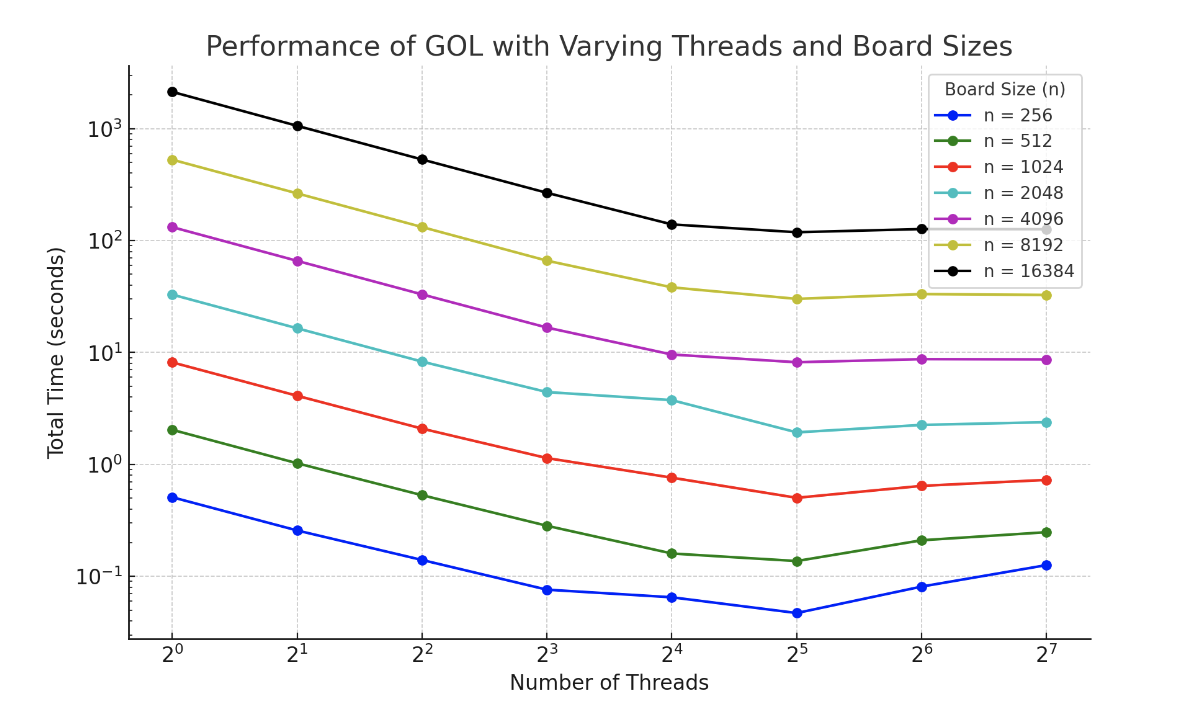
\includegraphics[width=0.5\textwidth]{pthreads.png}
    \caption{Performance of Pthreads implementation of Game of Life}
    \label{fig:pthreads}
\end{figure}

First, we observed a direct correlation between the size of the board and the run-time; larger boards invariably required longer to process, highlighting the computational limitations of using traditional Pthreads for large-scale simulations. Second, an increase in the number of threads generally led to a reduction in run-time, demonstrating the benefits of parallel processing. However, this improvement in performance was not linear. Beyond 16 threads, the addition of more threads resulted in a performance plateau or in some cases a slight deterioration in efficiency. This phenomenon can be attributed to the overhead associated with managing a large number of threads and the diminishing returns of parallel processing on a fixed number of CPU cores. These results established a baseline for performance, critical for subsequent comparative analysis against the CUDA and MPI implementations of GOL.

\subsection{CUDA Experiments}

The CUDA-accelerated version of the GOL simulation will offload the computation to the GPU. For our tests, we used a machine that utilized an NVIDIA RTX A4000 graphics card, a very powerful single-slot GPU. We measured the execution time and resource usage and compared it to both the Pthreads and OpenMPI implementations, again using an automated git bash script. 

Our CUDA experiments were structured to evaluate the performance of the GOL simulation under various conditions, particularly focusing on the impact of different board sizes and iteration counts on the GPU's efficiency. We ran tests with board sizes ranging from 2,048 x 2,048 to 32,768 x 32,768 and iterations ranging from 128 to 1024, with both metrics incrementing by powers of two. This experiment structure enabled us to better understand GPU scalability with increasing computational demands while concurrently assessing how the GPU handles extended computational tasks. In addition to these tests, we also experimented with compiler optimization flags to probe potential performance enhancements, although these showed minimal impact. From our test results, it appears that the primary performance improvements were due to leveraging CUDA's system architecture and GPU capabilities. The results of our experiments are presented below in Figure 2.

\begin{figure}[!htbp]
    \centering
    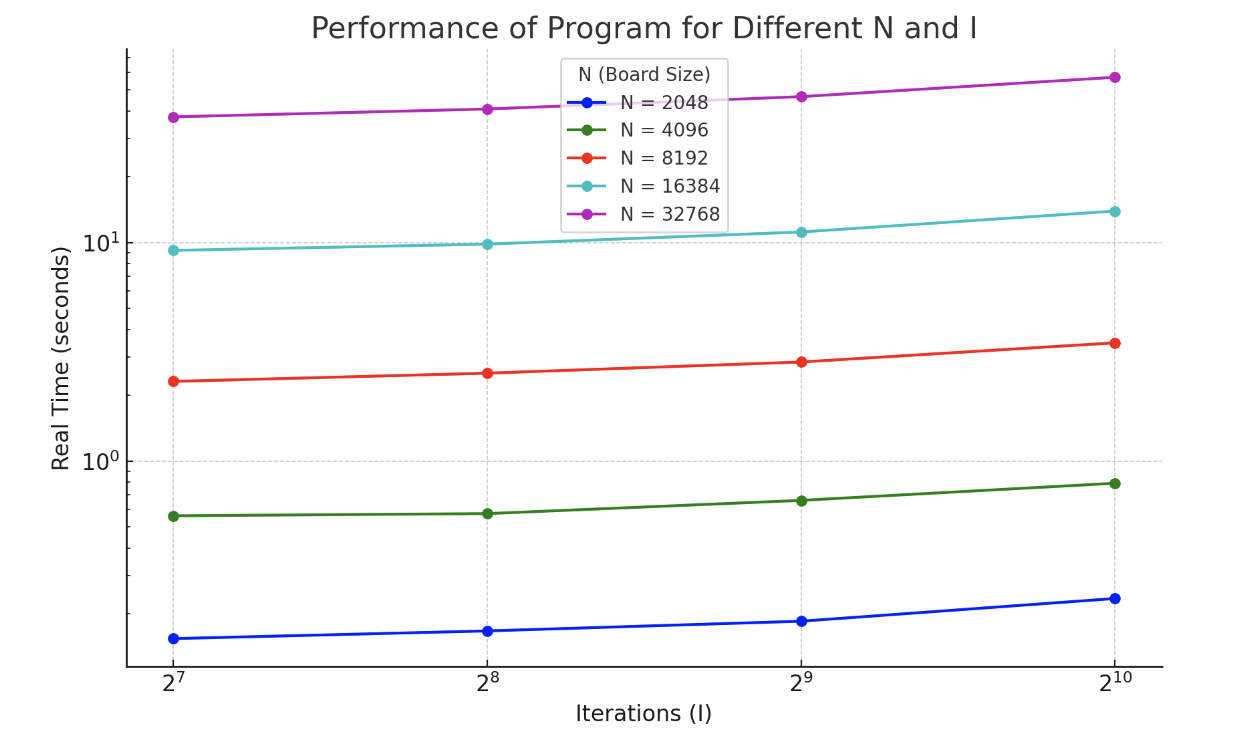
\includegraphics[width=0.5\textwidth]{cuda.png}
    \caption{Performance of CUDA implementation of Game of Life}
    \label{fig:cuda}
\end{figure}

Another critical aspect of our testing was determining the maximum board size that a single GPU could handle, which was found to be around 45,000 x 45,000. Our results indicate that above this board size there is not enough memory available in a single machine to be able to play a round of GOL. Figure 3 shows the results of attempting to allocate more memory than available in a single machine. To push the limits of the CUDA implementation further, we also conducted tests on larger boards, incrementing from 16,384 x 16,384 to 32,768 x 32,768, with iteration counts scaling from 1,024 to 4,096. These large-scale tests were helpful for understanding the performance boundaries of our CUDA implementation under extreme conditions and comparing to our OpenMPI and hybrid implementation performances.

\begin{figure}[!htbp]
    \centering
    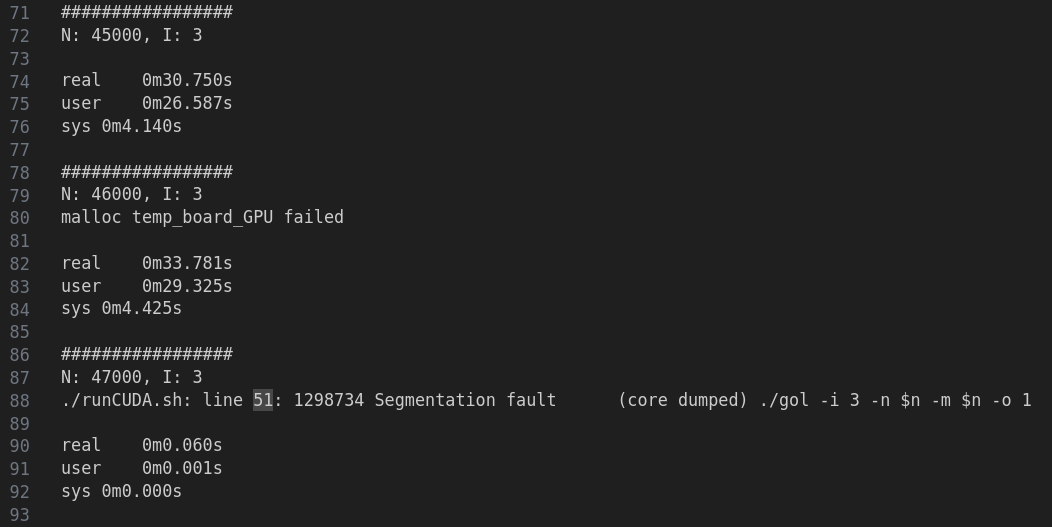
\includegraphics[width=0.5\textwidth]{CUDAExp3.png}
    \caption{Maximum board size limit for CUDA implementation}
    \label{fig:CUDAExp3}
\end{figure}

We observed that the GPU efficiently processed increasing board sizes up to the identified limit of 45,000 x 45,000, showcasing excellent processing power and a fair amount of scalability. An increase in iterations led to a gradual increase in computation time, demonstrating the GPU's capability to manage long-duration tasks effectively. In the large-scale tests, the GPU maintained robust performance, although run-times increased with the volume of computations, indicating a balance between computational load and available hardware resources.

Through this set of experiments, our CUDA implementation demonstrated its effectiveness in GPU-based parallel processing for large-scale simulations compared to our baseline Pthreads. For example, our Pthreads baseline experiment of a 16,384 x 16,384 board size with 128 iterations and an optimal 32 threads took 2 minutes and 11 seconds, while the CUDA equivalent experiment took 9.3 seconds (approximately 14 times faster).

\subsection{OpenMPI Experiments}

Our exploration into the OpenMPI experiments was driven by the objective of assessing the scalability of (GOL) in contexts where the board sizes were substantially larger than what a single GPU could manage. The intent was to harness the power of distributed computing via the OpenMPI interface, capitalizing on the cumulative computational capabilities of multiple CPU hosts. For our experiments, the largest number of host machines we used was 32. This setup was particularly crucial for understanding the performance dynamics when the computational load is distributed across various nodes, each handling a portion of the overall GOL board.

The experimental design we employed involved incrementally increasing the board sizes and observing how the system managed these sizes as more processes were introduced. Similar to our previous experiments, we automated the data collection process by using a git bash script. However, we held iterations constant at 128 to strictly observe the relation between board size, number of processes, and runtime, since increasing the number of iterations is guaranteed to increase the overall runtime. The setup was calibrated to ensure that each host's CPU efficiently computed segments of the game board, with a particular focus on the synchronization of overlapping sections (ghost cells) between different nodes. 

From our results in Figure 4 we noted a consistent decrease in runtime as the number of processes increased, affirming the effectiveness of distributed computing. However, this efficiency gain was more pronounced with larger board sizes. For smaller boards, the addition of more processes did not significantly improve runtime, and in some cases, it introduced resource wastage and contention. This finding suggests that while OpenMPI is adept at handling larger simulations by distributing the workload evenly, its advantage diminishes with smaller problem sizes where the overhead of managing multiple processes outweighs the benefits.

\begin{figure}[!htbp]
    \centering
    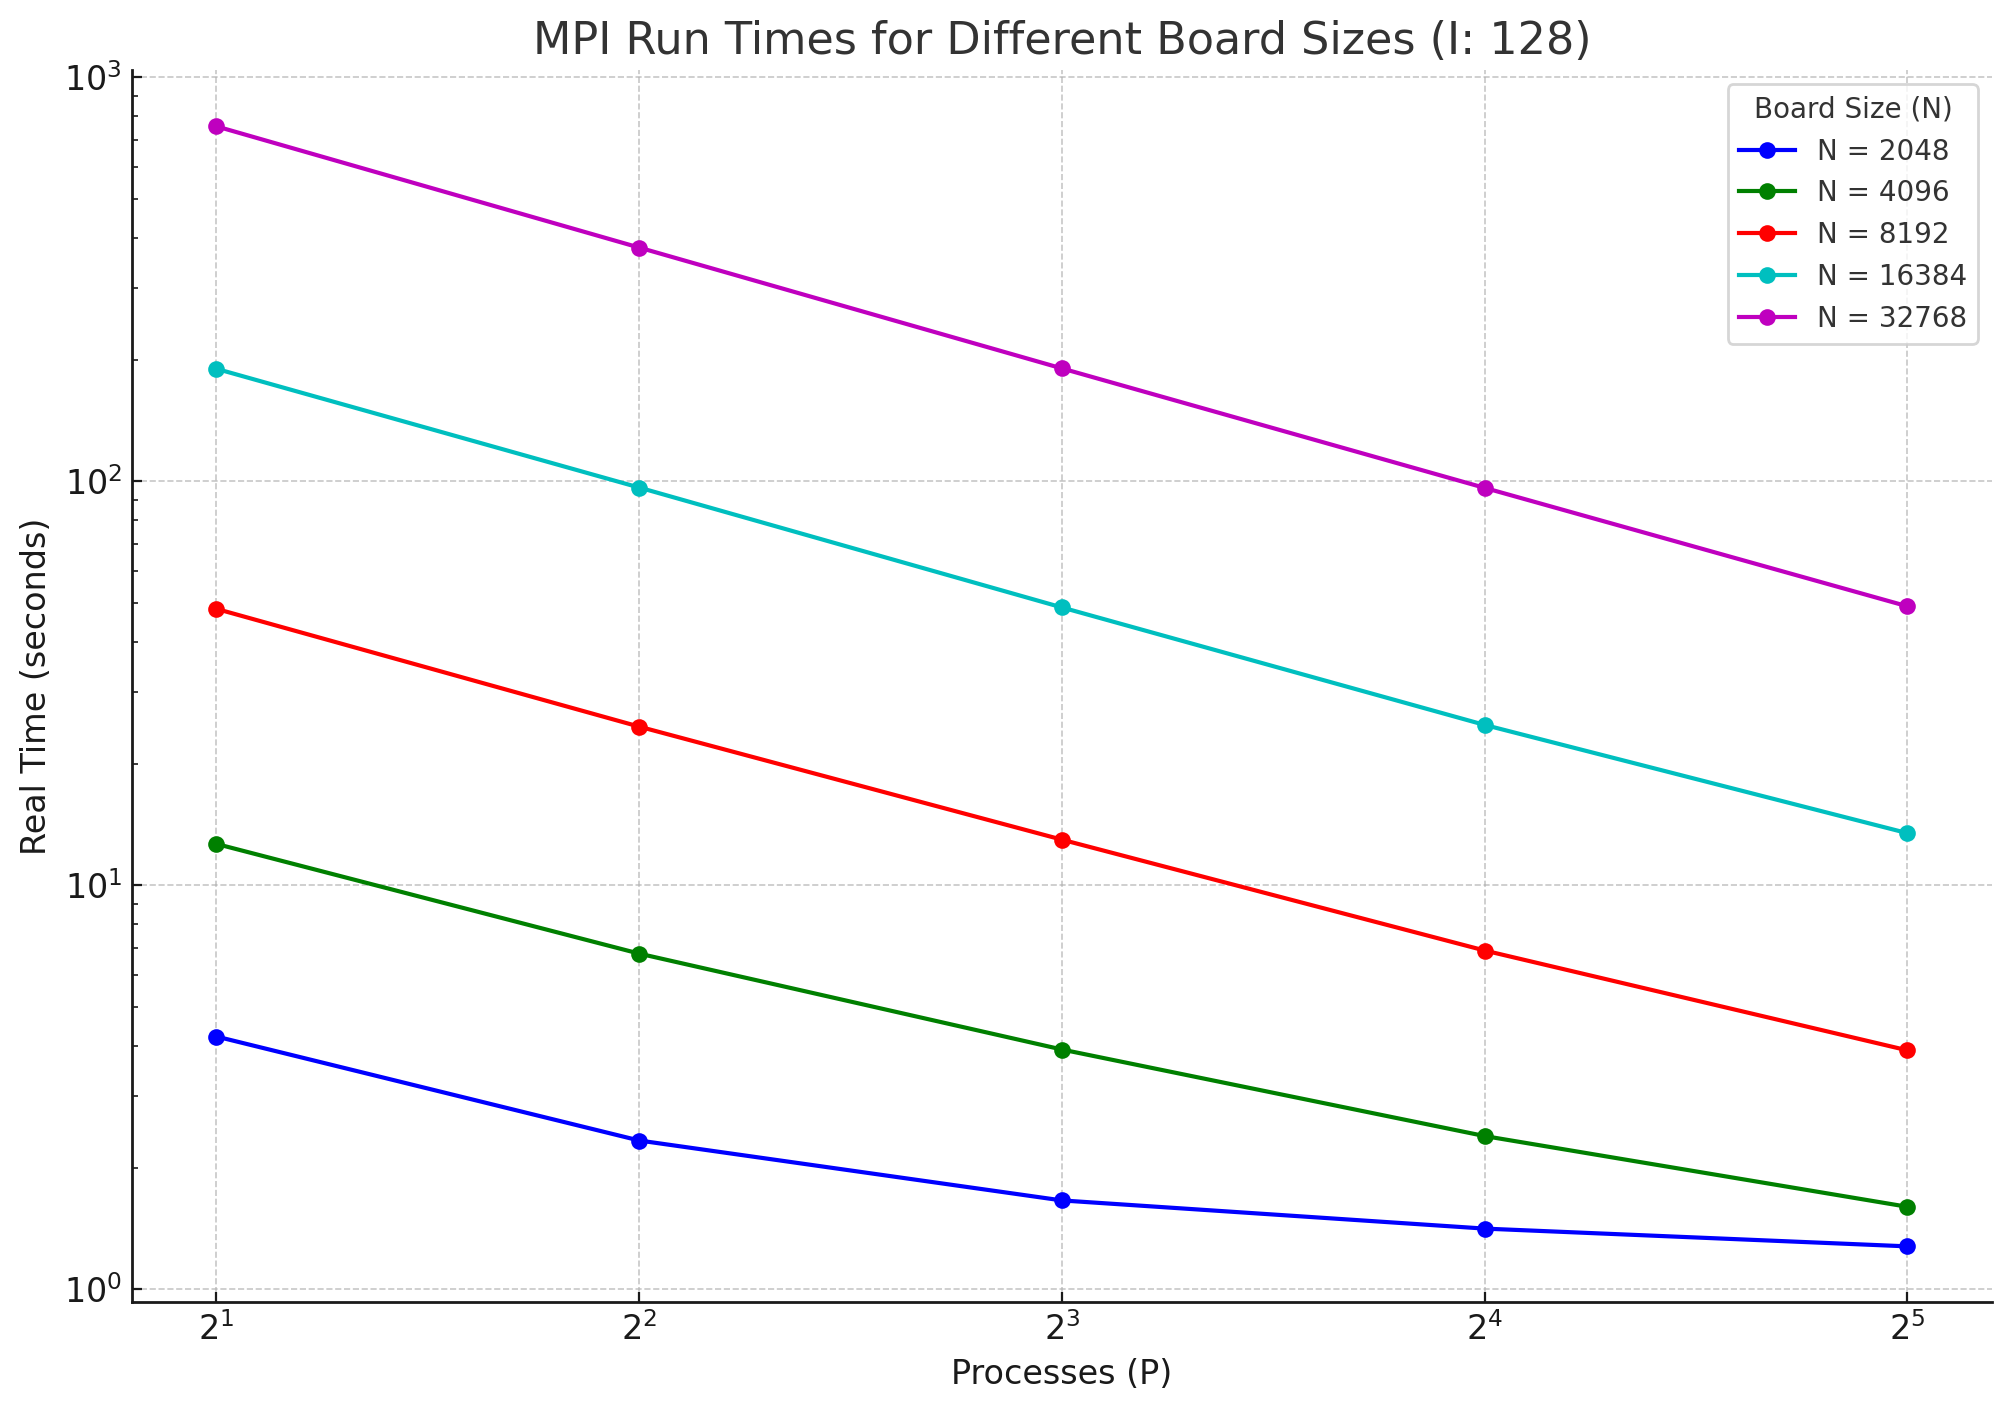
\includegraphics[width=0.5\textwidth]{newMPI.png}
    \caption{Performance of OpenMPI implementation of Game of Life}
    \label{fig:mpi}
\end{figure}

We also wanted to test the limits of our OpenMPI implementation, and thus designed two experiments -- one to increment board sizes up until the same memory allocation errors occurred as in our CUDA experiments, and one for a large size board (32,000 x 32,000) with a large amount of iterations (1024 and 2048). Figure 5 indicates that above a 262,144 x 262,144 board size there is not enough memory available in a single machine to be able to play a round of GOL even after dividing the overall board into 32 segments for each machine to process. This again supports our notion of the effectiveness of distributed computing, since our OpenMPI implementation could handle board sizes nearly 8 times larger than our CUDA implementation.

\begin{figure}[!htbp]
    \centering
    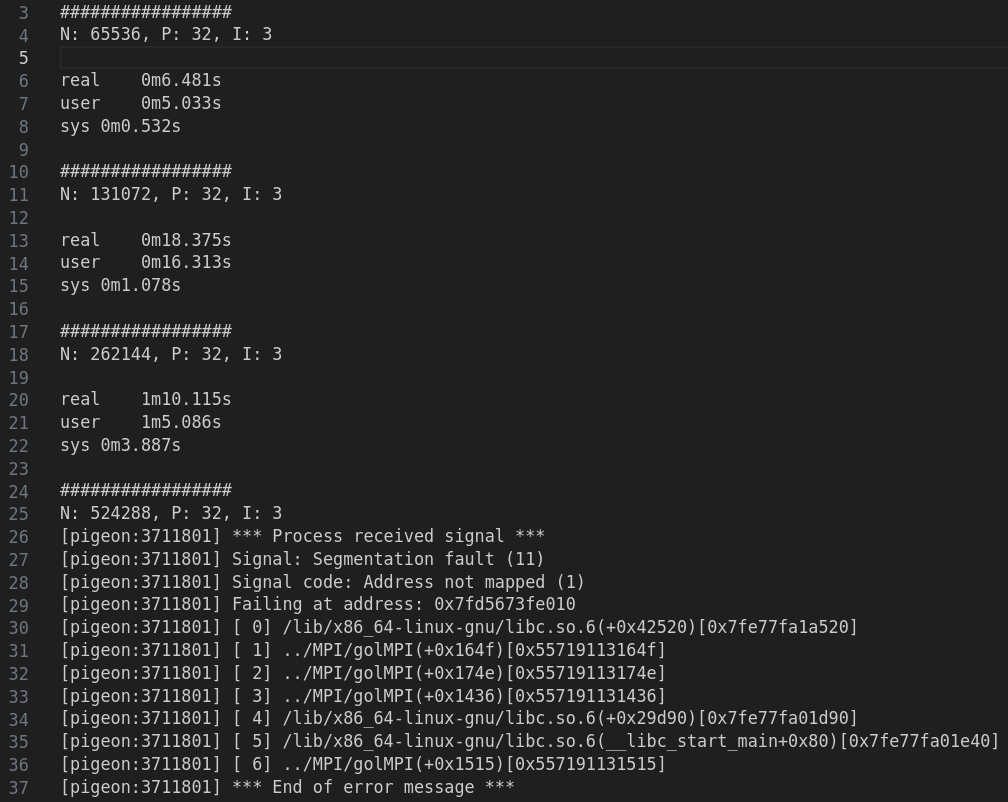
\includegraphics[width=0.5\textwidth]{MPIExp2.png}
    \caption{Maximum board size limit for MPI implementation}
    \label{fig:MPIExp2}
\end{figure}

In essence, these experiments underscored the pivotal role of problem size in distributed computing. The optimal utilization of OpenMPI's capabilities is heavily dependent on the nature and scale of the task at hand. Larger problems benefit immensely from the distributed approach, demonstrating capability where other implementations fail. In contrast, smaller tasks might not reap the same level of benefits, highlighting the importance of aligning computational strategy with problem characteristics. These insights are crucial for understanding the applicability and efficiency of distributed computing models in various simulation scenarios.

\subsection{CUDA-OpenMPI Experiments}

To showcase the combined benefits of MPI and CUDA, we integrated both parallelization methodologies. This time, we limited our experimental analysis to a board size of 32,000 x 32,000 (the upper end of board sizes for our CUDA implementation) and incremented iterations from 1024 to 2048. This experiment structure allows us to easily compare runtime performance across all three implementations, as we have previously obtained results for large scale, large iteration experiments for both CUDA and OpenMPI. Our primary objective with this experiment was to keep all factors the same across all three implementations and observe runtime performance of each to see if our hybrid model provided any significant benefit over the individual CUDA and OpenMPI implementations. We also performed a singular test of a board size of 65,536 x 65,356 to ensure that our hybrid model could handle board sizes outside the range that CUDA could handle. We discuss our results of this experiment in the next section. 

\subsection{Comparative Analysis}

In our comprehensive study, we undertook a series of experiments to assess the efficiency and scalability of four distinct parallel programming models: traditional Pthreads, CUDA, OpenMPI, and our hybrid model. Each of these models provide their own unique benefits, but through our experiments we aimed to determine the most efficient approach for different problem sizes and computational environments. Figure 6 presents the runtime performance of traditional Pthreads, CUDA, and OpenMPI implementations as board size doubles. Note that the most optimal value of 32 threads are used to obtain these Pthreads results, and the most optimal number of 32 processes are used to obtain these OpenMPI results.  

The Pthreads implementation, serving as our baseline, was tested across various board sizes and thread counts. We observed that while Pthreads offered some degree of parallel processing efficiency, it was significantly outperformed in both speed and scalability by the other two models. This outcome highlighted the limitations of traditional CPU-based multithreading, especially when dealing with large-scale simulations.

In contrast, CUDA showcased remarkable computational efficiency, capitalizing on the parallel processing prowess of GPUs. As board size increased, CUDA’s ability to leverage thousands of threads on a GPU translated to unparalleled computational speed. 

\begin{figure}[!htbp]
    \centering
    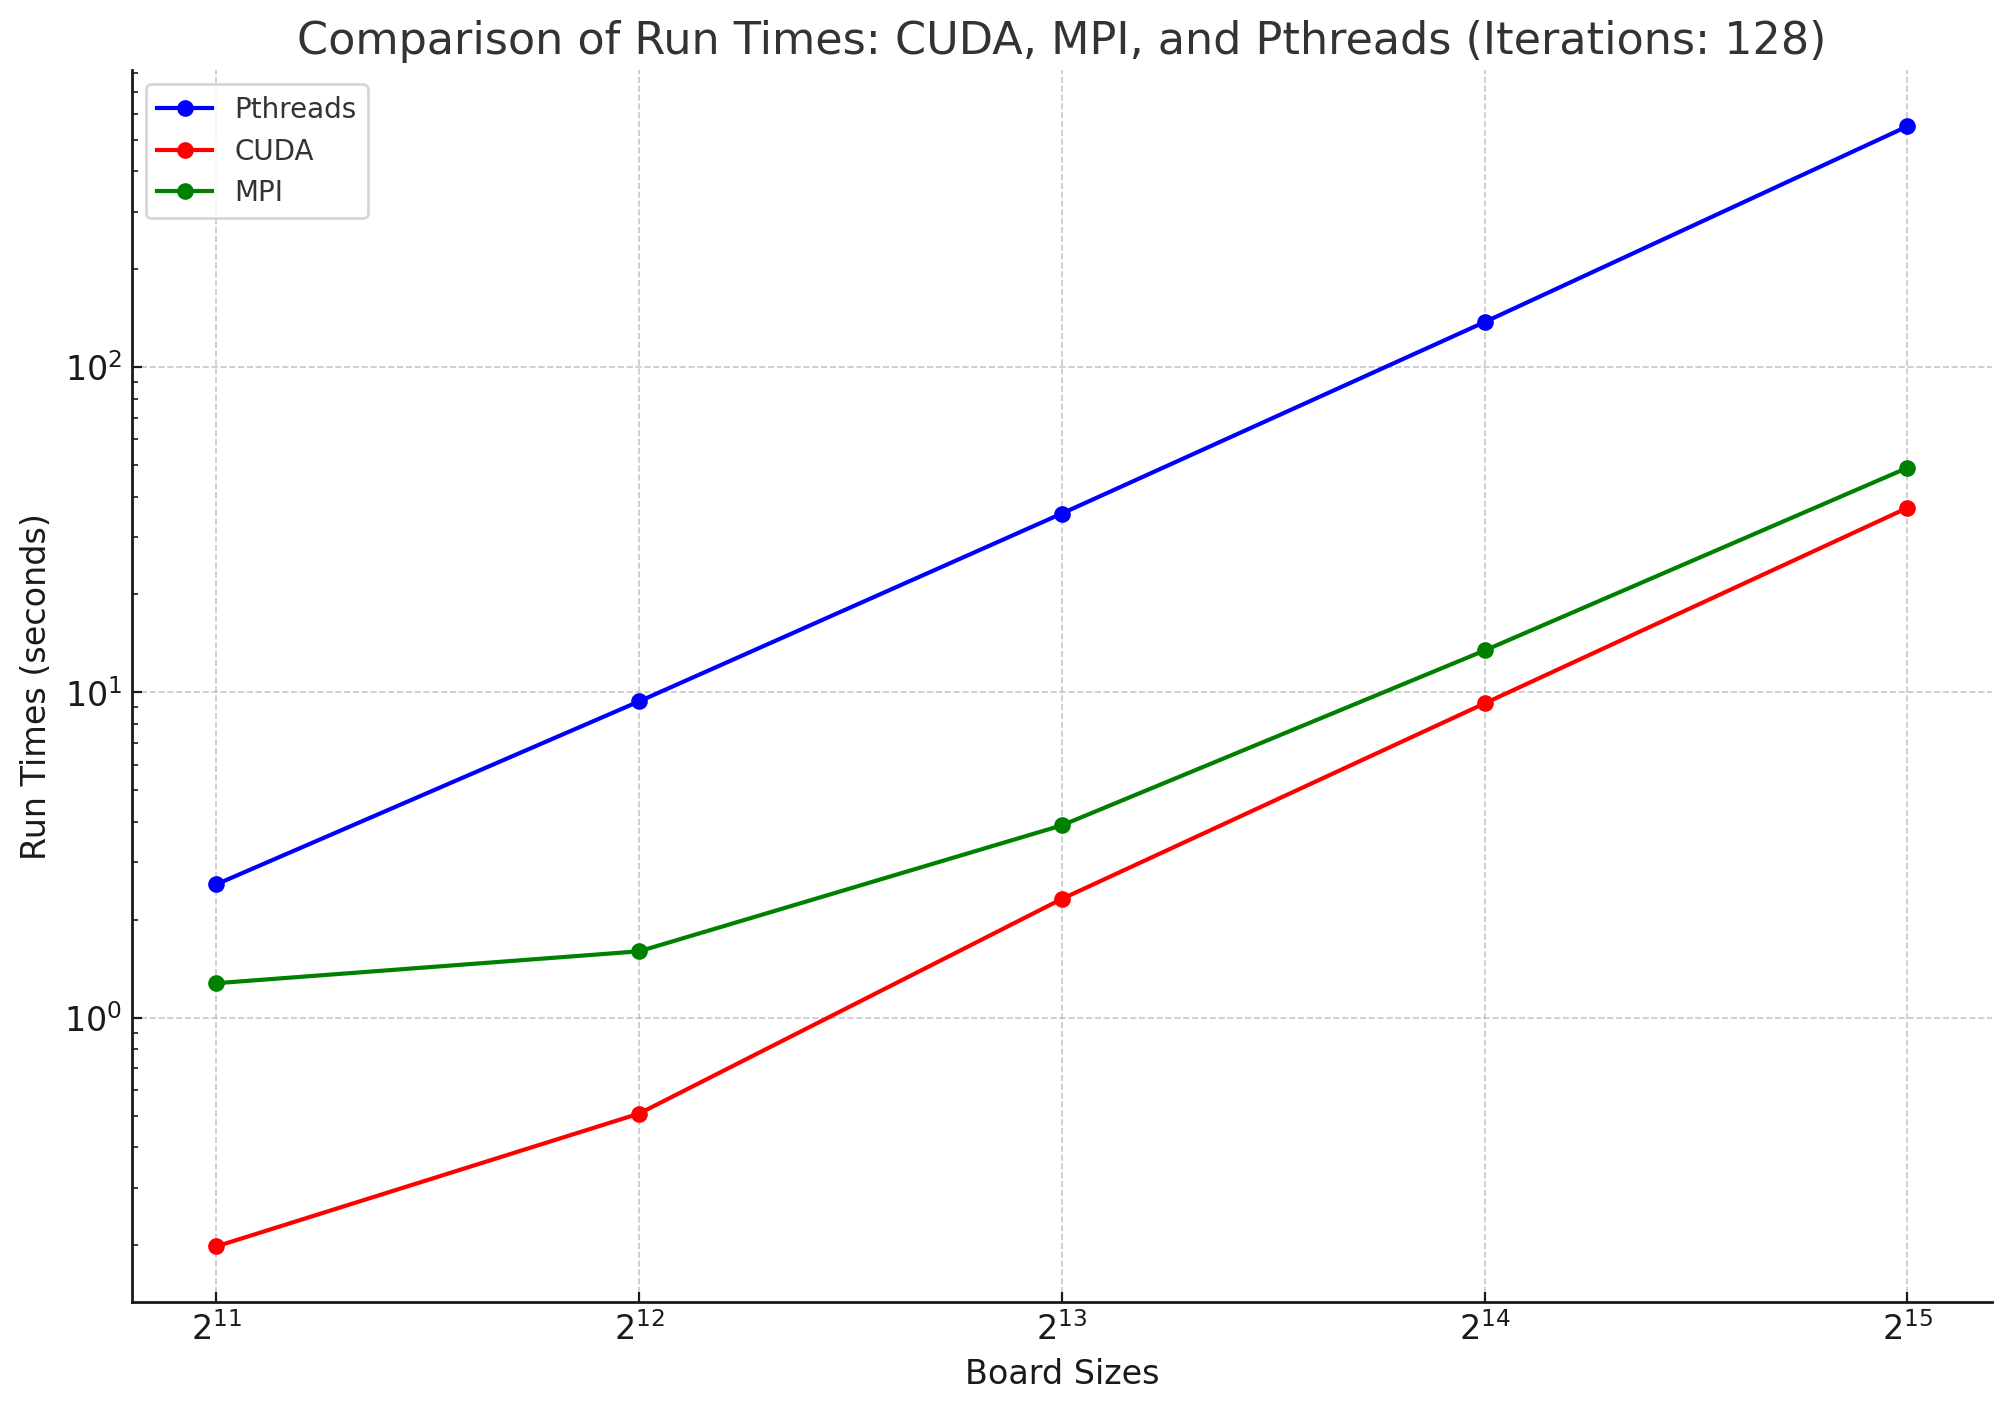
\includegraphics[width=0.5\textwidth]{newComp.png}
    \caption{Performance of Pthreads, CUDA, and OpenMPI implementation of Game of Life.}
    \label{fig:comp}
\end{figure}

On the other hand, while OpenMPI exhibited superior scalability compared to Pthreads, particularly in handling larger problem sizes, it fell short of achieving the peak computational speeds that CUDA is known for. For all board sizes ranging from 2,048 x 2,048 to 32,768 x 32,768, CUDA outperformed even the most optimized Pthreads and OpenMPI implementations for the same amount of 128 iterations. This discrepancy in performance can be attributed to the inherent architectural differences between the two frameworks. OpenMPI excels in distributing computational tasks across multiple CPUs within a network, effectively managing simulations that are too expansive for a single GPU's capacity. However, it lacks the specialized parallel processing capabilities that CUDA leverages through GPUs. CUDA's design allows it to perform a high volume of simultaneous calculations, exploiting the massive parallelism of GPU cores. 

Now, we compare our CUDA and OpenMPI results to the results of our hybrid model implementation. Figure 7 presents a table of our results for large scale iterations on a 32,000 x 32,000 board, with both OpenMPI and our hybrid model utilizing 32 processes. We observed that OpenMPI significantly underperformed the CUDA and hybrid implementations for large iterations, which aligns with our expectations since the OpenMPI model accrues significant performance drawbacks due to the overhead of having to pass information across nodes every single round.
\begin{figure}[!htbp]
    \centering
    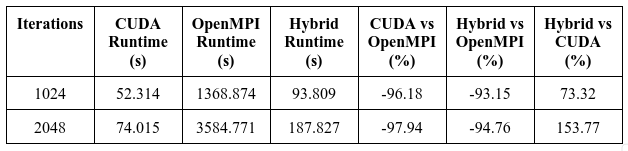
\includegraphics[width=0.5\textwidth]{CompAnalysis.png}
    \caption{Runtime performance of 32,000 x 32,000 board for CUDA, OpenMPI, and hybrid models}
    \label{fig:CompAnalysis}
\end{figure}

We also observed that our hybrid model performed surprisingly well, with runtimes that were clearly slower than CUDA but significantly faster than OpenMPI. As expected, CUDA performs the best for board sizes that it can handle due to the GPU's impressive processing power and the lack of overhead in message passing across nodes. 

\section{Conclusions}
% Conclusions and Future Directions for your work Conclude with the main ideas
% and results of your work. Discuss ways in which your project could be
% extended...what's next? what are the interesting problems and questions that
% resulted from your work?
Through our experimentation and investigation of the performance enhancement capabilities of DES using a hybrid MPI-CUDA model, we found that there is significant room for improvement in adapting and optimizing such a hybrid model. Our results show that this hybrid MPI-CUDA model adequately leverages the benefits of both GPU-acceleration and distributed computing, while not being impacted by the typical limitations of either model. It can handle larger board sizes than a single GPU can manage, while not being significantly slowed down by the overhead of message passing. Though not shown in our results, we can expect that as the number of iterations increases even further the runtime performance between CUDA and the other two models will diverge even further since more rounds of GOL simulation will slow down the MPI models more than it will slow down the CUDA model. Our research in this paper underscores the significance of offloading CPU-intensive tasks to the GPU and how drastically it can improve application performance. 

In the future it would be good to fix our data transfer issues in our hybrid model, as we have yet to ascertain if the data being sent across nodes is fully correct. In our hybrid model we have only guaranteed that there is a successful transfer of information and that there are GOL calculations/ processing being performed every round, but not that the data being processed on the boundary of each processes' local grid is valid. We have only verified that data that lies anywhere other than the top and bottom rows of each local grid is playing GOL correctly as per the game rules.

It would also be nice to experiment further with ghost cell optimization, as both our OpenMPI and hybrid implementations only passed information about the very top and very bottom rows of its portion of the grid to neighboring processes. Increasing or decreasing the amount of rows being sent may or may not improve overall performance, since more information being sent less frequently may or may not be faster than less information being sent more frequently. 

\section{Meta-discussion}\label{meta} 
% A brief meta-discussion of your project Include two paragraphs in this section:
% Discussion of what you found to be the most difficult and least difficult parts
% of your project.  In what ways did your implementation vary from your proposal
% and why?  
Completing this project was a lot more work than any of us had envisioned, and working through some of the challenges proved to be quite difficult. One of the most difficult parts of this project was when we were working through our CUDA implementation and had to keep track of which variables the CPU had access to, which variables the GPU had access to, and how/ when to send information from one memory system to the other. This was a meticulous process, but once we figured it out our hybrid model which utilized CUDA became a lot easier to implement. We also had difficulty in deciphering the MPI syntax, as the functions that MPI use have a significant amount of parameters that need to be adjusted and interpreted correctly. Again, once we figured out the syntax the structure of our implementation was easy to code.

In our proposal we aimed to do a lot more incremental testing, but this did not turn out to be the case. We should have practiced better modular design as we were writing up our CUDA and OpenMPI implementations, and tried some small runs as we went. We only added a print board function very late into the development process, and in hindsight would have been more useful for debugging than for verifying our CUDA and OpenMPI solutions were correct at the end. Our OpenMPI and hybrid implementations also differed from our proposal in that there was no ghost cell optimization being performed like we had originally planned. Time constraints and longer than expected debugging prevented us from exploring that route for our project. 
% The References section is auto generated by specifying the .bib file
% containing bibtex entries, and the style I want to use (plain)
% compiling with latex, bibtex, latex, latex, will populate this
% section with all references from the .bib file that I cite in this paper
% and will set the citations in the prose to the numbered entry here
\bibliography{finalreport}
\bibliographystyle{plain}

\end{document}